\section{System Model and Problem Formulation}
\label{sec:problem-formulation}

\subsection{System Model}
\label{sec:system-model}

An instructional program is produced by a harness that wraps a language model
(\cref{fig:architecture}). The model generates content; the harness owns the
state, the workflow, and the quality control. The central state is a versioned
\emph{alignment graph} that every module reads or writes.

\begin{figure*}[t]
  \centering
  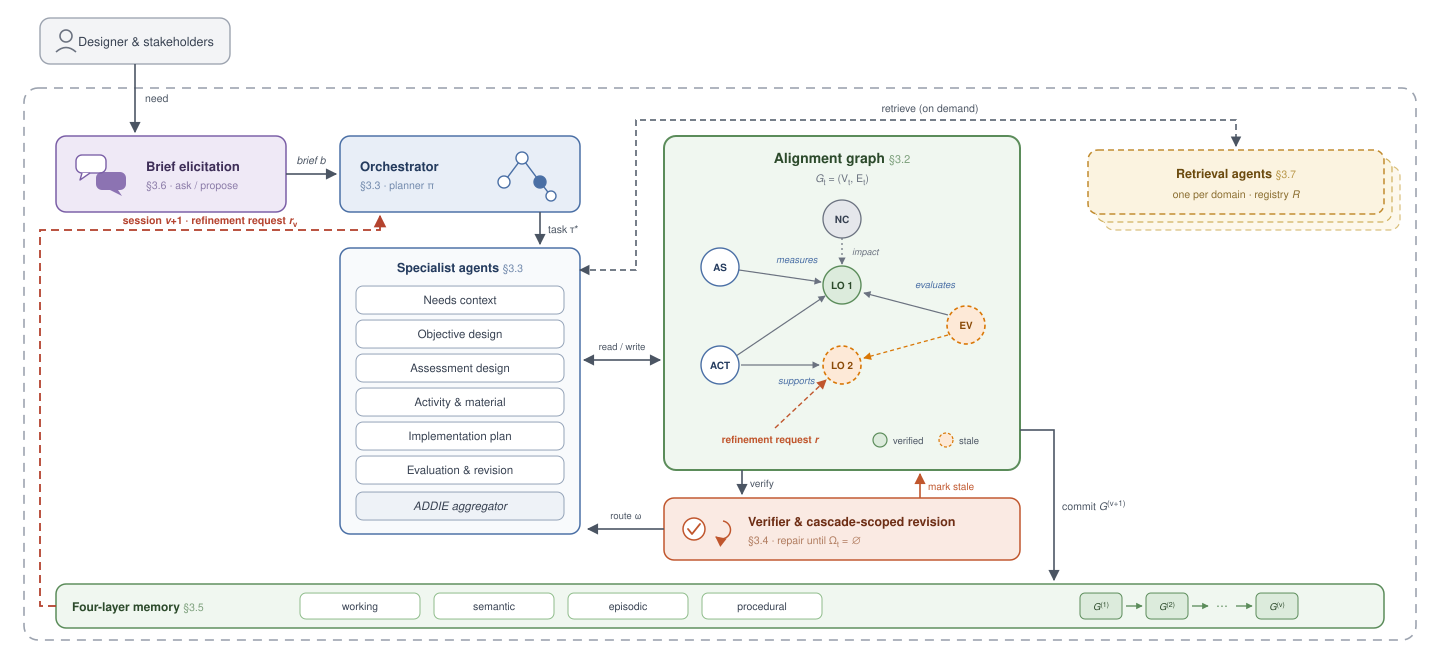
\includegraphics[width=\textwidth]{figures/architecture}
  \caption{Architecture of AlignmentGraph-ISD. Specialist agents run in a fixed
  instructional-design order (top), each writing only its own node/edge types
  into the versioned alignment graph at the center. After writing, a specialist
  runs pedagogical verification and repair as a tool within its turn (self-check
  loop). A final aggregator emits the ADDIE program and records a silent residual
  audit. The model is interchangeable (LLM or SLM); every mechanism belongs to the
  harness.}
  \label{fig:architecture}
\end{figure*}

\subsection{The Alignment Graph}
\label{sec:alignment-graph}

The root difficulty is that the relations among design components exist only
implicitly in text: a reader may \emph{sense} that an assessment measures an
objective, but the system cannot check it. AlignmentGraph-ISD reifies constructive
alignment~\cite{biggs1996enhancing} as an explicit data structure. At each step
$t$, the design state is a graph $G_t = (V_t, E_t)$ whose vertices cover the
artifacts of all five ADDIE phases:
\begin{multline*}
V_t = V_{\mathrm{needs}} \cup V_{\mathrm{objective}} \cup V_{\mathrm{assessment}} \cup V_{\mathrm{activity}} \\
 \cup V_{\mathrm{material}} \cup V_{\mathrm{implementation}} \cup V_{\mathrm{evaluation}}.
\end{multline*}
The edge set is kept minimal: three many-to-many relations centered on objectives,
\begin{align*}
E_t &= E_{\mathrm{measures}} \cup E_{\mathrm{supports}} \cup E_{\mathrm{evaluates}},\\
E_{\mathrm{measures}} &\subseteq V_{\mathrm{assessment}} \times V_{\mathrm{objective}},\\
E_{\mathrm{supports}} &\subseteq V_{\mathrm{activity}} \times V_{\mathrm{objective}},\\
E_{\mathrm{evaluates}} &\subseteq V_{\mathrm{evaluation}} \times V_{\mathrm{objective}}.
\end{align*}
A \textsl{measures} edge pairs an assessment with an objective it grades, a
\textsl{supports} edge pairs an activity with an objective it practices, and an
\textsl{evaluates} edge pairs an evaluation item with an objective it appraises.
Only objectives are decomposed into element nodes per learning outcome
(\texttt{objective:LO-*}), because alignment must be checked per objective. An
objective is \emph{aligned} if and only if at least one assessment measures it, one
activity supports it, and one evaluation evaluates it: for all $o \in V_{\mathrm{objective}}$,
\begin{multline}
\label{eq:aligned}
\mathrm{aligned}(o) \iff \big(\exists a\colon (a,o) \in E_{\mathrm{measures}}\big) \\
 \wedge \big(\exists x\colon (x,o) \in E_{\mathrm{supports}}\big) \wedge \big(\exists e\colon (e,o) \in E_{\mathrm{evaluates}}\big).
\end{multline}
\Cref{eq:aligned} is the operational definition of constructive alignment in the
system; the harness's task is to make it hold for every objective, and to make
each edge \emph{valid}---an assessment that genuinely elicits the objective's
cognitive level, not merely a link that exists. Each node carries a \texttt{stale}
flag and \texttt{repair\_history}; each edge a \texttt{verified} flag---these are
the fields that make alignment measurable in \cref{sec:results}.

\subsection{Notation and Assumptions}
\label{sec:assumptions}

\Cref{tab:notation} lists the notation. We assume: (i) a design brief $b$ is given
(brief formation is out of scope; see \cref{sec:threats-limitations}); (ii) the
model is stateless and interchangeable---no mechanism relies on a specific model
or on model capability beyond following instructions; (iii) the output must
conform to the ADDIE schema of the benchmark, so ADDIE serves as the output
contract, not as an execution constraint.

\begin{table}[t]
  \caption{Notation.}
  \label{tab:notation}
  \small
  \begin{tabular}{@{}ll@{}}
    \toprule
    Symbol & Meaning \\
    \midrule
    $b$ & design brief (harness input) \\
    $G_t=(V_t,E_t)$ & alignment graph at step $t$ \\
    $o \in V_{\mathrm{objective}}$ & a learning objective (element node) \\
    $\mathrm{aligned}(o)$ & constructive-alignment predicate, \cref{eq:aligned} \\
    $A_i$ & specialist agent for ISD concern $i$ \\
    $V^{(i)},E^{(i)}$ & node/edge types agent $i$ may write \\
    $\mathcal{V}$ & pedagogical verifier; $\Omega=\mathcal{V}(G)$ its violations \\
    \bottomrule
  \end{tabular}
\end{table}

\subsection{Problem Statement}
\label{sec:problem-statement}

Given a design brief $b$, produce a complete instructional program---i.e.\ a graph
$G$ and its rendered ADDIE artifacts---such that
\begin{enumerate}
  \item[(i)] every learning objective is aligned in the sense of \cref{eq:aligned},
  with each edge \emph{valid} at the objective's intended cognitive level
  (constructive alignment); and
  \item[(ii)] this quality is guaranteed by the harness rather than by the raw
  capability of the model---i.e.\ it is preserved as the model is scaled down from
  an LLM to an SLM.
\end{enumerate}

\subsection{Challenges}
\label{sec:challenges}

Three properties make the problem hard. \emph{Cross-artifact coupling}: condition
(i) is relational, so no single agent that sees only its own artifact can certify
it. \emph{Invisibility}: a violation of (i) does not surface as a local error---the
prose looks fine---so it must be detected structurally, not by inspection.
\emph{Model independence}: condition (ii) forbids relying on model capability, so
the guarantee must come from checkable state and explicit control, which is
exactly what a prompt-only agent lacks.
